\subsection*{Đề thi thử THPTQG 2026 - Lần 2 - Trường THPT chuyên Khoa Học Tự Nhiên - Hà Nội }
\Opensolutionfile{ans}[ans/ans-OTTNTHPT-DE28-LC]

\caulc

\begin{ex}%[2H5N2-2]
Trong không gian với hệ toạ độ $Oxyz$, cho phương trình đường thẳng $d \colon \begin{cases} x = 3 - 2t \\ y = -1 + 2t \\ z = 2 - t \end{cases}$ ($t \in \mathbb{R}$). Vectơ nào sau đây là một vectơ chỉ phương của đường thẳng $d$?
\choice
{\True $\vec{u}_1=(-2;2;-1)$}
{$\vec{u}_2=(3;-1;2)$}
{$\vec{u}_3=(2;-2;-1)$}
{$\vec{u}_4=(-2;-1;-1)$}
\loigiai{
	Đường thẳng $d$ có phương trình tham số $\begin{cases} x = 3 - 2t \\ y = -1 + 2t \\ z = 2 - t \end{cases}$ nên nhận vectơ $\vec{u}=(-2;2;-1)$ làm một vectơ chỉ phương.
}
\end{ex}

\begin{ex}%[2D1H4-1]
Đường tiệm cận xiên của đồ thị hàm số $y=\dfrac{-5x^{2}+3x+1}{x-1}$ có phương trình là
\choice
{$y=5x+2$}
{$y=-5x+2$}
{$y=-5-2x$}
{\True $y=-5x-2$}
\loigiai{
	Thực hiện phép chia đa thức, ta có:
	$$
	y = \dfrac{-5x^2+3x+1}{x-1} = \dfrac{-5x(x-1) - 2(x-1) - 1}{x-1} = -5x - 2 - \dfrac{1}{x-1}.
	$$
	Vì $\lim\limits_{x \to \infty} \left(y - (-5x-2)\right) = \lim\limits_{x \to \infty} \left(-\dfrac{1}{x-1}\right) = 0$ nên đường tiệm cận xiên của đồ thị hàm số là $y = -5x - 2$.
}
\end{ex}

\begin{ex}%[1D1N5-3]
Tập nghiệm của phương trình $\cos x = 1$ là
\choice
{$S=\left\{\dfrac{\pi}{2}+k2\pi \ \middle| \ k \in \mathbb{Z}\right\}$}
{\True $S=\left\{k2\pi \ \middle| \ k \in \mathbb{Z}\right\}$}
{$S=\left\{k\pi \ \middle| \ k \in \mathbb{Z}\right\}$}
{$S=\left\{\dfrac{\pi}{2}+k\pi \ \middle| \ k \in \mathbb{Z}\right\}$}
\loigiai{
	Phương trình $\cos x = 1 \Leftrightarrow x = k2\pi$ ($k \in \mathbb{Z}$). 
	Vậy tập nghiệm là $S=\left\{k2\pi \ \middle| \ k \in \mathbb{Z}\right\}$.
}
\end{ex}

\begin{ex}%[1D6H4-3]
Tập nghiệm của bất phương trình $\log_{\frac{1}{2}}(2x-5) \ge 1$ là
\choice
{$\left(\dfrac{5}{2};\dfrac{11}{4}\right)$}
{\True $\left(\dfrac{5}{2};\dfrac{11}{4}\right]$}
{$\left(\dfrac{11}{4};+\infty\right)$}
{$\left[\dfrac{11}{4};+\infty\right)$}
\loigiai{
	Điều kiện: $2x - 5 > 0 \Leftrightarrow x > \dfrac{5}{2}$.
	$$
	\log_{\frac{1}{2}}(2x-5) \ge 1 \Leftrightarrow 2x - 5 \le \left(\dfrac{1}{2}\right)^1 \Leftrightarrow 2x \le \dfrac{11}{2} \Leftrightarrow x \le \dfrac{11}{4}.
	$$
	Kết hợp với điều kiện, ta được tập nghiệm $S = \left(\dfrac{5}{2};\dfrac{11}{4}\right]$.
}
\end{ex}

\begin{ex}%[1H8H1-3]
Cho hình chóp $S.ABCD$ có đáy là hình vuông cạnh $a$. Cạnh bên $SA$ vuông góc với mặt phẳng đáy, $SA = a$. Độ lớn của góc $\widehat{BSD}$ bằng
\choice
{$120^\circ$}
{$45^\circ$}
{$90^\circ$}
{\True $60^\circ$}
\loigiai{
	Đáy $ABCD$ là hình vuông cạnh $a$ nên $BD = a\sqrt{2}$.\\
	Vì $SA \perp (ABCD)$ nên các tam giác $SAB, SAD$ vuông tại $A$. Suy ra:
	$$
	SB = \sqrt{SA^2 + AB^2} = \sqrt{a^2 + a^2} = a\sqrt{2}.
	$$
	$$
	SD = \sqrt{SA^2 + AD^2} = \sqrt{a^2 + a^2} = a\sqrt{2}.
	$$
	Xét tam giác $SBD$ có $SB = SD = BD = a\sqrt{2}$ nên tam giác $SBD$ là tam giác đều. \\
	Vậy $\widehat{BSD} = 60^\circ$.
}
\end{ex}

\begin{ex}%[2H5H1-3]
Trong không gian với hệ tọa độ $Oxyz$, cho $3$ điểm $A(1;3;5)$, $B(2;1;0)$, $C(-2;0;3)$. Phương trình mặt phẳng $(ABC)$ là
\choice
{\True $11x-17y+9z-5=0$}
{$11x-17y+9z+5=0$}
{$11x+17y-9z+5=0$}
{$17x+11y-9z+5=0$}
\loigiai{
	Ta có $\vec{AB} = (1; -2; -5)$ và $\vec{AC} = (-3; -3; -2)$.\\
	Vectơ pháp tuyến của mặt phẳng $(ABC)$ là $\vec{n} = [\vec{AB}, \vec{AC}] = (-11; 17; -9)$.\\
	Phương trình mặt phẳng $(ABC)$ đi qua $A(1;3;5)$ là:
	$$
	-11(x - 1) + 17(y - 3) - 9(z - 5) = 0 \Leftrightarrow -11x + 17y - 9z + 5 = 0 \Leftrightarrow 11x - 17y + 9z - 5 = 0.
	$$
}
\end{ex}

\begin{ex}%[2D6H1-2]
Cho hai biến cố $A, B$ sao cho $\mathrm{P}(A)=0{,}5$; $\mathrm{P}(B)=0{,}4$; $\mathrm{P}(A|B)=0{,}3$. Khi đó $\mathrm{P}(B|A)$ bằng
\choice
{$\dfrac{3}{25}$}
{$\dfrac{4}{25}$}
{\True $\dfrac{6}{25}$}
{$\dfrac{1}{5}$}
\loigiai{
	Ta có $\mathrm{P}(A \cap B) = \mathrm{P}(B) \cdot \mathrm{P}(A|B) = 0{,}4 \cdot 0{,}3 = 0{,}12$.\\
	Xác suất điều kiện $\mathrm{P}(B|A)$ là:
	$$
	\mathrm{P}(B|A) = \dfrac{\mathrm{P}(A \cap B)}{\mathrm{P}(A)} = \dfrac{0{,}12}{0{,}5} = 0{,}24 = \dfrac{6}{25}.
	$$
}
\end{ex}

\begin{ex}%[2D4H2-2]
Biết $\displaystyle\int\limits_{1}^{2}\dfrac{1}{2x^{2}+5x+3}\mathrm{\,d}x = \ln\dfrac{a}{b}$ với $a,b$ là các số nguyên lớn hơn $1$, phân số $\dfrac{a}{b}$ tối giản. Giá trị $T = a + b$ bằng
\choice
{$28$}
{\True $29$}
{$12$}
{$10$}
\loigiai{
	Ta phân tích mẫu số: $2x^2 + 5x + 3 = (x+1)(2x+3)$.
	$$
	\dfrac{1}{(x+1)(2x+3)} = \dfrac{1}{x+1} - \dfrac{2}{2x+3}.
	$$
	Khi đó:
	$$
	\displaystyle\int\limits_{1}^{2}\dfrac{1}{2x^{2}+5x+3}\mathrm{\,d}x = \int\limits_{1}^{2} \left( \dfrac{1}{x+1} - \dfrac{2}{2x+3} \right) \mathrm{\,d}x = \left[ \ln|x+1| - \ln|2x+3| \right]_{1}^{2}
	$$
	$$
	= (\ln 3 - \ln 7) - (\ln 2 - \ln 5) = \ln\dfrac{3}{7} - \ln\dfrac{2}{5} = \ln\dfrac{15}{14}.
	$$
	Suy ra $a = 15, b = 14$. Giá trị $T = 15 + 14 = 29$.
}
\end{ex}

\begin{ex}%[1D5H2-2]
Thống kê mức tiêu dùng của $20$ hộ gia đình hàng tháng có bảng số liệu sau
\begin{center}
\begin{tabular}{|l|c|c|c|c|c|}
\hline
\textbf{Chi phí tiêu dùng (triệu đồng)} & $[5;10)$ & $[10;15)$ & $[15;20)$ & $[20;25)$ & $[25;30)$ \\
\hline
\textbf{Số gia đình} & $1$ & $3$ & $8$ & $5$ & $3$ \\
\hline
\end{tabular}
\end{center}
Giá trị trung vị của mẫu số liệu trên bằng
\choice
{\True $18{,}75$}
{$18{,}25$}
{$18$}
{$13{,}75$}
\loigiai{
	Cỡ mẫu $n = 20$. Vị trí trung vị là $\dfrac{n}{2} = 10$.\\
	Tần số tích lũy của các nhóm lần lượt là: $1; 4; 12; 17; 20$.\\
	Vì $4 < 10 \le 12$ nên nhóm chứa trung vị là nhóm $[15; 20)$.\\
	Giá trị trung vị là:
	$$
	M_e = 15 + \dfrac{10 - 4}{8} \cdot 5 = 15 + \dfrac{6}{8} \cdot 5 = 18{,}75.
	$$
}
\end{ex}

\begin{ex}%[1D3H3-3]
Cho hàm số $f(x)=\dfrac{ax^{2}+2x-5}{x^{2}-3x+2}$ (với $a$ là hằng số). Biết rằng $f(x)$ liên tục tại điểm $x=1$. Giá trị của $f(1)$ bằng
\choice
{$-6$}
{\True $-8$}
{$2$}
{$3$}
\loigiai{
	Hàm số liên tục tại $x=1$ nên $\lim\limits_{x \to 1} f(x)$ tồn tại hữu hạn. \\
	Do mẫu $x^2 - 3x + 2 = 0$ tại $x=1$ nên tử số cũng phải bằng $0$ tại $x=1$:
	$$
	a(1)^2 + 2(1) - 5 = 0 \Leftrightarrow a = 3.
	$$
	Khi đó $f(x) = \dfrac{3x^2+2x-5}{x^2-3x+2} = \dfrac{(x-1)(3x+5)}{(x-1)(x-2)} = \dfrac{3x+5}{x-2}$ (với $x \neq 1$).\\
	Vậy $f(1) = \lim\limits_{x \to 1} \dfrac{3x+5}{x-2} = \dfrac{3(1)+5}{1-2} = -8$.
}
\end{ex}

\begin{ex}%[2D1H2-1]
Cho hàm số $y=f(x)$. Đồ thị hàm số $f'(x)$ là đồ thị một hàm số bậc 3 như hình vẽ bên.
\immini{
Số điểm cực tiểu của hàm số $y=f(x)$ là
\choice
{3}
{1}
{2}
{\True 0}
}{
\begin{tikzpicture}[>=stealth,scale=0.8]
\draw[->] (-2.5,0) -- (3.5,0) node[below] {$x$};
\draw[->] (0,-4.5) -- (0,1.5) node[left] {$y$};
\draw (0,0) node[below left] {$O$};
\draw[thick] plot[smooth,samples=100,domain=-1.2:2.5] (\x, {-(\x+1)*(\x-2)*(\x-2)});
\fill (-1,0) circle (2pt) node[above left] {-1};
\fill (2,0) circle (2pt) node[above] {2};
\fill (0,-4) circle (2pt) node[left] {-4};
\end{tikzpicture}
}
\loigiai{
Dựa vào đồ thị $f'(x)$, ta thấy $f'(x)=0$ tại $x=-1$ và $x=2$.
\begin{itemize}
    \item Tại $x=-1$, $f'(x)$ đổi dấu từ dương sang âm nên hàm số đạt cực đại tại $x=-1$.
    \item Tại $x=2$, $f'(x)$ không đổi dấu (đồ thị tiếp xúc với trục hoành và nằm phía dưới trục hoành ở lân cận điểm đó) nên $x=2$ không phải là điểm cực trị.
\end{itemize}
Vậy hàm số không có điểm cực tiểu nào.
}
\end{ex}

\begin{ex}%[1D2V3-8]
\immini{
Một hình vuông có cạnh bằng $3$. Chia hình vuông đó thành $9$ hình vuông bằng nhau và tô màu hình vuông ở chính giữa. Với mỗi hình vuông nhỏ chưa được tô màu, lại chia thành $9$ hình vuông bằng nhau và tô màu hình vuông ở chính giữa. Cứ như thế, quá trình trên được lặp lại. Diện tích phần được tô màu sau $3$ lần chia bằng
\choice
{\True $\dfrac{217}{81}$}
{$\dfrac{161}{81}$}
{$\dfrac{217}{729}$}
{$\dfrac{512}{81}$}
}{
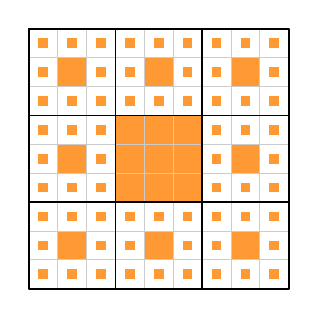
\begin{tikzpicture}[line join=round, line cap=round, >=stealth, scale=1.1]
    \draw[fill=white] (0,0) rectangle (3,3);
    \fill[orange!80] (1,1) rectangle (2,2);
    \foreach \x in {0, 1, 2} {
        \foreach \y in {0, 1, 2} {
            \pgfmathparse{\x==1 && \y==1 ? 1 : 0}
            \ifnum\pgfmathresult=0
                \fill[orange!80] (\x+1/3, \y+1/3) rectangle (\x+2/3, \y+2/3);
            \fi
        }
    }
    \foreach \x in {0, 1, 2} {
        \foreach \y in {0, 1, 2} {
            \pgfmathparse{\x==1 && \y==1 ? 1 : 0}
            \ifnum\pgfmathresult=0
                \foreach \xx in {0, 1, 2} {
                    \foreach \yy in {0, 1, 2} {
                        \pgfmathparse{\xx==1 && \yy==1 ? 1 : 0}
                        \ifnum\pgfmathresult=0
                            \fill[orange!80] (\x+\xx/3+1/9, \y+\yy/3+1/9) rectangle (\x+\xx/3+2/9, \y+\yy/3+2/9);
                        \fi
                    }
                }
            \fi
        }
    }
    \draw[step=1/3, gray!40, very thin] (0,0) grid (3,3);
    \draw[step=1, black, thin] (0,0) grid (3,3);
    \draw[thick] (0,0) rectangle (3,3);
\end{tikzpicture}
}
\loigiai{
	Diện tích ban đầu của hình vuông là $S = 3^2 = 9$.\\
	- Lần $1$: Tô màu $\dfrac{1}{9}$ diện tích, phần tô màu là $S_1 = 9 \cdot \dfrac{1}{9} = 1$. Diện tích còn lại là $8$.\\
	- Lần $2$: Tô màu $\dfrac{1}{9}$ diện tích còn lại, phần tô màu là $S_2 = 8 \cdot \dfrac{1}{9} = \dfrac{8}{9}$. Diện tích còn lại là $8 - \dfrac{8}{9} = \dfrac{64}{9}$.\\
	- Lần $3$: Tô màu $\dfrac{1}{9}$ diện tích còn lại, phần tô màu là $S_3 = \dfrac{64}{9} \cdot \dfrac{1}{9} = \dfrac{64}{81}$.\\
	Tổng diện tích được tô màu sau 3 lần là:
	$$
	S = S_1 + S_2 + S_3 = 1 + \dfrac{8}{9} + \dfrac{64}{81} = \dfrac{81 + 72 + 64}{81} = \dfrac{217}{81}.
	$$
}
\end{ex}

\cauds

\begin{ex}%[2D6V1-4]
Một thư viện thực hiện khảo sát $200$ độc giả chia làm hai nhóm tuổi: nhóm trẻ (dưới $35$ tuổi) và nhóm trung niên (từ $35$ tuổi trở lên). Các độc giả chỉ lựa chọn đọc $1$ trong $3$ loại sách: văn học, khoa học và ẩm thực. Kết quả thu được cho thấy: có $120$ người thuộc nhóm trẻ. Có $80$ người lựa chọn đọc sách văn học. Số người thuộc nhóm trung niên lựa chọn đọc sách khoa học là $20$ người. Biết rằng hai biến cố `độc giả thuộc nhóm trung niên' và `độc giả lựa chọn đọc sách văn học' là hai biến cố độc lập. Chọn ngẫu nhiên một độc giả được khảo sát.
\choiceTF
{\True Xác suất để độc giả được chọn là thuộc nhóm trẻ bằng $0{,}6$.}
{Xác suất để độc giả được chọn là trung niên và đọc sách văn học là $0{,}2$.}
{\True Trong số các độc giả lựa chọn sách văn học, có đúng $48$ người thuộc nhóm trẻ.}
{\True Biết rằng người được chọn thuộc nhóm trung niên, xác suất để người đó đọc sách ẩm thực là $35\%$.}
\loigiai{
	Ký hiệu $T$: nhóm trẻ, $TN$: nhóm trung niên. $V$: sách văn học, $K$: sách khoa học, $A$: sách ẩm thực. Tổng số $N=200$.\\
	$n(T) = 120 \Rightarrow n(TN) = 200 - 120 = 80$. Do đó $\mathrm{P}(TN) = \dfrac{80}{200} = 0{,}4$.\\
	$n(V) = 80 \Rightarrow \mathrm{P}(V) = \dfrac{80}{200} = 0{,}4$.\\
	$TN$ và $V$ độc lập nên $\mathrm{P}(TN \cap V) = \mathrm{P}(TN) \cdot \mathrm{P}(V) = 0{,}4 \cdot 0{,}4 = 0{,}16$. Số người trung niên đọc văn học là $0{,}16 \cdot 200 = 32$.\\
	Nhóm trung niên có $80$ người, trong đó đọc văn học ($32$), khoa học ($20$), nên đọc ẩm thực là $n(TN \cap A) = 80 - 32 - 20 = 28$.\\
	Số người trẻ đọc văn học là $n(T \cap V) = n(V) - n(TN \cap V) = 80 - 32 = 48$.
	\begin{itemchoice}
		\itemch Đúng. Xác suất chọn được nhóm trẻ là $\mathrm{P}(T) = \dfrac{120}{200} = 0{,}6$.
		\itemch Sai. Xác suất trung niên đọc văn học là $\mathrm{P}(TN \cap V) = 0{,}16 \neq 0{,}2$.
		\itemch Đúng. Số lượng nhóm trẻ đọc văn học là $n(T \cap V) = 48$.
		\itemch Đúng. Xác suất đọc sách ẩm thực với điều kiện nhóm trung niên là $\mathrm{P}(A|TN) = \dfrac{28}{80} = 0{,}35 = 35\%$.
	\end{itemchoice}
}
\end{ex}

\begin{ex}%[1D6V3-5]
Một nhóm nghiên cứu quan sát sự phát triển của một quần thể vi khuẩn trong môi trường nuôi cấy hạn chế. Giai đoạn $1$ (từ $t=0$ đến $t=3$ giờ): Số lượng vi khuẩn tăng trưởng theo hàm mũ $N(t)=50\mathrm{e}^{0{,}8t}$ (với $t$ tính bằng giờ, $N$ tính bằng triệu cá thể). Giai đoạn $2$ (sau $3$ giờ): Do nguồn dinh dưỡng cạn kiệt, tốc độ tăng trưởng giảm dần. Từ thời điểm này, số lượng vi khuẩn lúc này tuân theo hàm số $M(t)=A-B\mathrm{e}^{-0{,}6t}$. Biết quá trình phát triển là liên tục và trơn (vận tốc phát triển liên tục).
\choiceTF
{\True Số lượng vi khuẩn tại thời điểm bắt đầu là $50$ triệu cá thể.}
{\True Tốc độ tăng trưởng của vi khuẩn tại thời điểm $t=3$ lớn hơn $440$ triệu cá thể/giờ.}
{Giá trị $B = \dfrac{200}{3}$.}
{Số lượng vi khuẩn tối đa (ngưỡng bão hòa) mà môi trường này có thể duy trì là $1285$ triệu cá thể (kết quả làm tròn đến hàng đơn vị).}
\loigiai{
	Tốc độ tăng trưởng ở GĐ 1: $N'(t) = 50 \cdot 0{,}8\mathrm{e}^{0{,}8t} = 40\mathrm{e}^{0{,}8t}$.\\
	Tốc độ tăng trưởng ở GĐ 2: $M'(t) = 0{,}6B\mathrm{e}^{-0{,}6t}$.\\
	Tính liên tục và trơn tại $t=3$ suy ra $N(3)=M(3)$ và $N'(3)=M'(3)$.
	\begin{itemchoice}
		\itemch Đúng. Tại $t=0$, $N(0) = 50\mathrm{e}^{0} = 50$ (triệu).
		\itemch Đúng. $N'(3) = 40\mathrm{e}^{2{,}4} \approx 440{,}92 > 440$.
		\itemch Sai. Ta có $M'(3) = N'(3) \Leftrightarrow 0{,}6B\mathrm{e}^{-1{,}8} = 40\mathrm{e}^{2{,}4} \Leftrightarrow B = \dfrac{200}{3}\mathrm{e}^{4{,}2} \neq \dfrac{200}{3}$.
		\itemch Sai. Số lượng tối đa là $\lim\limits_{t \to +\infty} M(t) = A$.\\
		Từ $N(3) = M(3) \Leftrightarrow 50\mathrm{e}^{2{,}4} = A - B\mathrm{e}^{-1{,}8} \Leftrightarrow A = 50\mathrm{e}^{2{,}4} + \left(\dfrac{200}{3}\mathrm{e}^{4{,}2}\right)\mathrm{e}^{-1{,}8} = \dfrac{350}{3}\mathrm{e}^{2{,}4} \approx 1286$ (chứ không phải 1285).
	\end{itemchoice}
}
\end{ex}

\begin{ex}%[2H5V4-4]
Trong không gian $Oxyz$, cho mặt cầu $(S) \colon (x+1)^{2}+(y-2)^{2}+(z-1)^{2}=9$ và điểm $A(1;-2;5)$.
\choiceTF
{Mặt cầu $(S)$ có tâm $I(-1;2;-1)$ và bán kính $R=3$.}
{\True Điểm $A$ nằm ngoài mặt cầu.}
{\True Phương trình mặt phẳng tiếp xúc với mặt cầu $(S)$ tại $T(-2;0;3)$ là $x+2y-2z+8=0$.}
{Xét các điểm $M$ thuộc $(S)$ sao cho đường thẳng $AM$ tiếp xúc với $(S)$, điểm $M$ luôn thuộc một mặt phẳng cố định có phương trình là $2x-4y+4z+3=0$.}
\loigiai{
	Mặt cầu $(S)$ có tâm $I(-1;2;1)$ và bán kính $R=3$.
	\begin{itemchoice}
		\itemch Sai. Tâm $I(-1;2;1)$, không phải $I(-1;2;-1)$.
		\itemch Đúng. Tính $IA = \sqrt{(1+1)^2 + (-2-2)^2 + (5-1)^2} = \sqrt{4+16+16} = 6 > R=3$.
		\itemch Đúng. Điểm $T(-2;0;3) \in (S)$. Vectơ pháp tuyến $\vec{IT} = (-1; -2; 2)$. Phương trình tiếp diện: $-1(x+2) - 2(y-0) + 2(z-3) = 0 \Leftrightarrow x+2y-2z+8=0$.
		\itemch Sai. Tập hợp tiếp điểm $M$ nằm trên mặt phẳng đối cực của điểm $A$ đối với $(S)$. Phương trình: $(x_A-x_I)(x-x_I) + (y_A-y_I)(y-y_I) + (z_A-z_I)(z-z_I) = R^2 \Leftrightarrow 2(x+1) - 4(y-2) + 4(z-1) = 9 \Leftrightarrow 2x - 4y + 4z - 3 = 0$. (Phương trình ở đề có $+3=0$ là sai).
	\end{itemchoice}
}
\end{ex}

\begin{ex}%[2D4V3-2]
\immini{
Cho đồ thị biểu diễn vận tốc của hai xe $A$ và $B$ khởi hành cùng một lúc, bên cạnh nhau và trên cùng một con đường. Biết đồ thị biểu diễn vận tốc của xe $A$ là $v_{A}(t)$ (km/h) một đường parabol, đồ thị biểu diễn vận tốc của xe $B$ là một đường thẳng $v_{B}(t)$ (km/h) ở hình bên.
\choiceTF
{Phương trình vận tốc của xe $B$ là $v_{B}(t)=15t$.}
{\True Vận tốc lớn nhất của xe $A$ trong $4$ giờ đầu di chuyển là $80$ km/h.}
{Quãng đường xe $A$ đi được trong $3$ giờ đầu là $120$ km.}
{Khoảng cách lớn nhất giữa hai xe trong $4$ giờ đầu di chuyển là $\dfrac{160}{3}$ km.}
}{
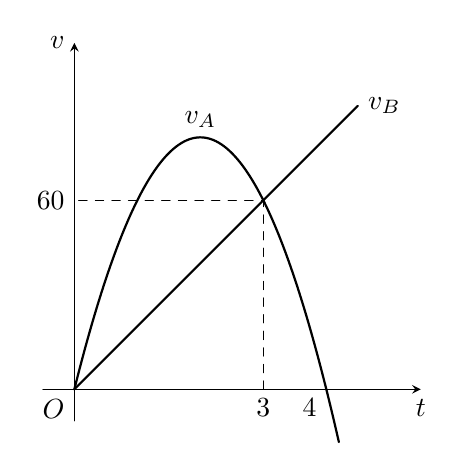
\begin{tikzpicture}[line join=round, line cap=round, >=stealth, scale=0.8]
    \coordinate (O) at (0,0);
    \draw[->] (-0.5,0) -- (5.5,0) node[below] {$t$};
    \draw[->] (0,-0.5) -- (0,5.5) node[left] {$v$};
    \node[below left] at (O) {$O$};
    \draw[smooth, samples=100, domain=0:4.2, thick] plot (\x, {-\x^2 + 4*\x});
    \node[above] at (2, 4) {$v_A$}; 
    \draw[thick] (0,0) -- (4.5,4.5) node[right] {$v_B$};
    \draw[dashed, thin] (3,0) node[below]{$3$} -- (3,3) -- (0,3) node[left]{$60$};
    \coordinate (M) at (3,3);
    \tkzDrawPoints[fill=black](M)
    \node[below left] at (4,0) {$4$};
    \coordinate (N) at (4,0);
    \tkzDrawPoints[fill=black](N)
\end{tikzpicture}
}
\loigiai{
	Theo đồ thị, tại $t=3$ thì $v = 60$, tức là trục tung có tỷ lệ $1$ đơn vị hình vẽ ứng với $20$ km/h. \\
	Hàm số $v_B(t)$ là đường thẳng đi qua gốc tọa độ nên $v_B(t) = kt$. Tại $t=3$, $v_B = 60 \Rightarrow k = 20$. Vậy $v_B(t) = 20t$.\\
	Hàm số $v_A(t)$ là Parabol đi qua $(0;0)$ và $(4;0)$ nên có dạng $v_A(t) = at(t-4)$. Đỉnh Parabol (trên hình vẽ) có tung độ là $4$ đơn vị, ứng với $v = 80$ km/h tại $t=2$. Suy ra $a(2)(-2) = 80 \Rightarrow a = -20$. Vậy $v_A(t) = -20t^2 + 80t$.
	\begin{itemchoice}
		\itemch Sai. $v_B(t) = 20t$.
		\itemch Đúng. Đỉnh parabol của $v_A$ tại $t=2$ có giá trị $80$ km/h.
		\itemch Sai. Quãng đường xe $A$ đi được trong 3 giờ là $S_A = \displaystyle\int\limits_0^3 (-20t^2+80t)\mathrm{\,d}t = \left[-\dfrac{20}{3}t^3 + 40t^2\right]_0^3 = 180$ km.
		\itemch Sai. Khoảng cách hai xe: $d(t) = \displaystyle\int\limits_0^t (v_A - v_B)\mathrm{\,d}x = -\dfrac{20}{3}t^3 + 30t^2$. Max đạt được khi $v_A = v_B \Leftrightarrow t=3$. Khi đó $d(3) = 90$ km.
	\end{itemchoice}
}
\end{ex}

\caukq

\begin{ex}%[1H8V6-1]
Cho hình chóp tam giác $S.ABC$ có đáy $ABC$ là tam giác vuông tại $B$, cạnh bên $SA$ vuông góc với mặt phẳng đáy. Biết $AB=\sqrt{3}$, $BC=1$ và góc giữa mặt phẳng $(SBC)$ và mặt phẳng $(ABC)$ bằng $60^\circ$. Tang của góc giữa đường thẳng $SC$ và mặt phẳng $(ABC)$ bằng bao nhiêu?
\loigiai{
\shortans{$1{,}5$}
\immini{
Vì $SA \perp (ABC)$ và $BC \perp AB$ (đáy vuông tại $B$) nên $BC \perp (SAB)$.\\
Giao tuyến của $(SBC)$ và $(ABC)$ là $BC$. Ta có $AB \perp BC$ và $SB \perp BC$, suy ra góc giữa hai mặt phẳng $(SBC)$ và $(ABC)$ là $\widehat{SBA}=60^\circ$.\\
Độ dài $SA=AB \cdot \tan 60^\circ = \sqrt{3} \cdot \sqrt{3} = 3$.\\
Góc giữa $SC$ và mặt phẳng $(ABC)$ là góc $\widehat{SCA}$.\\
Ta có $AC = \sqrt{AB^2+BC^2} = \sqrt{3+1} = 2$.\\
Vậy $\tan \widehat{SCA} = \dfrac{SA}{AC} = \dfrac{3}{2} = 1{,}5$.
}{
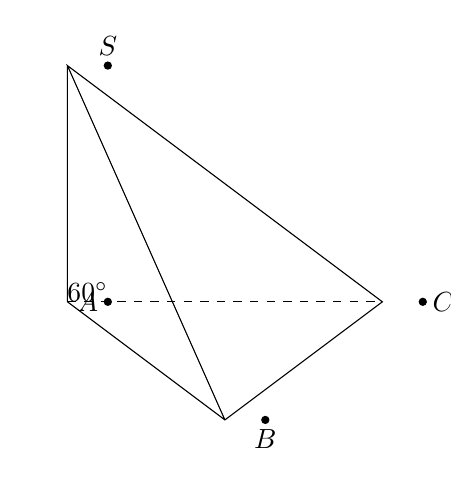
\begin{tikzpicture}[>=stealth,scale=1]
\def\a{2} \def\b{1.5} \def\h{3}
\coordinate (A) at (0,0);
\coordinate (B) at (\a,-\b);
\coordinate (C) at (2*\a,0);
\coordinate (S) at (0,\h);
\draw[dashed] (A) -- (C);
\draw (S) -- (A) -- (B) -- (C) -- (S) -- (B);
\tkzMarkRightAngle(A,B,C)
\tkzMarkRightAngle(S,A,B)
\tkzMarkRightAngle(S,A,C)
\tkzMarkAngle[size=0.6](S,B,A) \tkzLabelAngle[pos=0.9](S,B,A){$60^\circ$}
\tkzMarkAngle[size=0.8](S,C,A) 
\fill (S) circle (1.5pt) node[above] {$S$};
\fill (A) circle (1.5pt) node[left] {$A$};
\fill (B) circle (1.5pt) node[below] {$B$};
\fill (C) circle (1.5pt) node[right] {$C$};
\end{tikzpicture}
}
}
\end{ex}

\begin{ex}%[2D1V3-6]
\immini{
Nhân dịp No-en, gia đình bạn An cùng nhau trang trí nhà cửa. Tại góc phòng khách, bạn An dự kiến để một cây thông No-en ở vị trí $M$ cách hai bức tường lần lượt là $1$ m, $2$ m. Để cho căn phòng sáng hơn, bạn An sẽ lắp thêm dây đèn led $AB$ dưới sàn nhà, đi qua vị trí đặt cây thông, hai đầu dây đèn chạm vào tường. Độ dài dây đèn ngắn nhất bạn An cần dùng là bao nhiêu mét? (kết quả làm tròn đến hàng phần chục).
}{
\begin{tikzpicture}[line join=round, line cap=round, >=stealth, scale=1.4]
    \draw (0,0) rectangle (4,2.5);
    \draw[thick, blue] (1.3, 2.5) node[above, text=black]{$A$} -- (4, 1.2) node[right, text=black]{$B$};
    \coordinate (M) at (2.5, 1.92);
    \tkzDrawPoints[fill=black](M)
    \node[below left] at (M) {$M$};
    \draw[dashed, thin] (M) -- (2.5, 2.5) node[midway, right] {$1$ m};
    \draw[dashed, thin] (M) -- (4, 1.92) node[midway, below] {$2$ m};
\end{tikzpicture}
}
\shortans{$4{,}2$}
\loigiai{
	Chọn hệ tọa độ $Oxy$ với $O$ là góc phòng, hai bức tường là 2 trục $Ox, Oy$. Khi đó điểm $M(2; 1)$.\\
	Đường thẳng chứa dây đèn cắt $Ox$ tại $B(a;0)$ và $Oy$ tại $A(0;b)$ (với $a > 2, b > 1$).\\
	Phương trình đường thẳng $AB$: $\dfrac{x}{a} + \dfrac{y}{b} = 1$. Đi qua $M(2;1)$ nên $\dfrac{2}{a} + \dfrac{1}{b} = 1 \Rightarrow b = \dfrac{a}{a-2}$.\\
	Độ dài dây đèn là $L = \sqrt{a^2 + b^2}$. Ta cần tìm giá trị nhỏ nhất của $L^2 = a^2 + \dfrac{a^2}{(a-2)^2}$.\\
	Đặt $t = a - 2 > 0 \Rightarrow a = t + 2$. Khảo sát hàm số hoặc dùng Cauchy, chiều dài ngắn nhất của đoạn thẳng đi qua điểm $(p;q)$ cắt hai tia dương là $L_{\min} = \left( p^{2/3} + q^{2/3} \right)^{3/2}$.\\
	Áp dụng vào bài toán, ta có $L_{\min} = \left( 2^{2/3} + 1^{2/3} \right)^{3/2} \approx 4{,}1619$.\\
	Làm tròn đến hàng phần chục, ta được $4{,}2$ mét.
}
\end{ex}

\begin{ex}%[2D4C3-5]
\immini{
Trên mặt phẳng vẽ hai nửa đường tròn đường kính $AB, AD$, với $AB=2AD=4$ cm như hình vẽ. Cho biết $\widehat{BAC}=30^\circ$. Hình phẳng $(H)$ là phần tô đậm nằm giữa hai nửa đường tròn, đường thẳng $AB, AC$. Một kỹ sư cần chế tạo chi tiết máy bằng thép có dạng tròn xoay khi xoay hình phẳng $(H)$ quanh trục $AB$. Biết chi phí sản xuất là $15$ nghìn đồng/cm$^3$. Giá tiền sản xuất một chi tiết máy là bao nhiêu nghìn đồng? (kết quả làm tròn đến hàng đơn vị).
}{
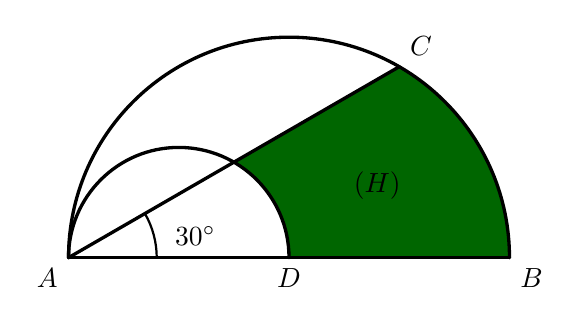
\begin{tikzpicture}[line join=round, line cap=round, >=stealth, scale=1.4, line width=1.2pt]
    \coordinate (A) at (0,0);
    \coordinate (D) at (2,0);
    \coordinate (B) at (4,0);
    \coordinate (C) at (3, {sqrt(3)});
    \coordinate (I) at (1.5, {sqrt(3)/2});
    \fill[green!40!black] 
        (2,0) -- (4,0) 
        arc (0:60:2) 
        -- (1.5, {sqrt(3)/2}) 
        arc (60:0:1) 
        -- cycle;
    \draw (4,0) arc (0:180:2);
    \draw (2,0) arc (0:180:1);
    \draw (0,0) -- (4,0);          
    \draw (0,0) -- (3, {sqrt(3)}); 
    \draw[line width=0.8pt] (0.8,0) arc (0:30:0.8);
    \node at (1.15, 0.2) {$30^\circ$};
    \node[below left] at (A) {$A$};
    \node[below] at (D) {$D$};
    \node[below right] at (B) {$B$};
    \node[above right] at (C) {$C$};
    \node at (2.8, 0.65) {$(H)$};
\end{tikzpicture}
}
\shortans{$192$}
\loigiai{
	Chọn hệ trục tọa độ $Oxy$ với $A$ trùng $O(0;0)$, $AB$ trùng $Ox$. Khi đó đường thẳng $AC$ có phương trình $y = \dfrac{x}{\sqrt{3}}$.\\
	Nửa đường tròn nhỏ đường kính $AD=2$ có phương trình $y_1 = \sqrt{2x - x^2}$.\\
	Nửa đường tròn lớn đường kính $AB=4$ có phương trình $y_2 = \sqrt{4x - x^2}$.\\
	Hoành độ giao điểm của $y = \dfrac{x}{\sqrt{3}}$ với $y_1$ là $x = 1{,}5$. Với $y_2$ là $x = 3$.\\
	Thể tích khối tròn xoay được tính theo công thức $V = V_1 + V_2 - V_3$, trong đó:
	$$
	V_1 = \pi \int\limits_{1{,}5}^{3} \left(\dfrac{x}{\sqrt{3}}\right)^2 \mathrm{\,d}x = \pi \left[ \dfrac{x^3}{9} \right]_{1{,}5}^{3} = \dfrac{21\pi}{8}
	$$
	$$
	V_2 = \pi \int\limits_{3}^{4} \left(4x-x^2\right) \mathrm{\,d}x = \pi \left[ 2x^2 - \dfrac{x^3}{3} \right]_{3}^{4} = \dfrac{5\pi}{3}
	$$
	$$
	V_3 = \pi \int\limits_{1{,}5}^{2} \left(2x-x^2\right) \mathrm{\,d}x = \pi \left[ x^2 - \dfrac{x^3}{3} \right]_{1{,}5}^{2} = \dfrac{5\pi}{24}
	$$
	Tổng thể tích $V = \dfrac{21\pi}{8} + \dfrac{5\pi}{3} - \dfrac{5\pi}{24} = \dfrac{49\pi}{12}$ cm$^3$.\\
	Giá tiền: $V \cdot 15 = \dfrac{49\pi}{12} \cdot 15 \approx 192{,}42$ nghìn đồng. Làm tròn đến hàng đơn vị là $192$.
}
\end{ex}

\begin{ex}%[2D6V2-4]
Trong giải đấu của trường, lớp 12A có lịch thi đấu hai trận vào thứ năm và chủ nhật. Xác suất lớp 12A thắng trận thứ năm là $40\%$, xác suất thắng trận chủ nhật là $50\%$. Khả năng thắng của đội phụ thuộc vào kết quả trận trước: nếu trận thứ năm thắng, xác suất thắng vào chủ nhật sẽ cao gấp ba lần so với trường hợp trận thứ năm thua. Xác suất để đội bóng lớp 12A thắng đúng một trận trong hai ngày đó là $\dfrac{a}{b}$ với $a,b$ là các số nguyên dương và $\dfrac{a}{b}$ tối giản. Giá trị $2a+b$ bằng bao nhiêu?
\shortans{$44$}
\loigiai{
	Gọi $W_1$ là biến cố thắng T5, $W_2$ là biến cố thắng CN. $L_1, L_2$ là các biến cố thua tương ứng.\\
	Theo bài ra: $\mathrm{P}(W_1) = 0{,}4 \Rightarrow \mathrm{P}(L_1) = 0{,}6$. Xác suất thắng tổng thể CN là $\mathrm{P}(W_2) = 0{,}5$.\\
	Đặt $\mathrm{P}(W_2 | L_1) = x \Rightarrow \mathrm{P}(W_2 | W_1) = 3x$.\\
	Ta có công thức xác suất toàn phần: $\mathrm{P}(W_2) = \mathrm{P}(W_1)\mathrm{P}(W_2|W_1) + \mathrm{P}(L_1)\mathrm{P}(W_2|L_1)$\\
	$\Leftrightarrow 0{,}5 = 0{,}4(3x) + 0{,}6(x) \Leftrightarrow 1{,}8x = 0{,}5 \Leftrightarrow x = \dfrac{5}{18}$.\\
	Xác suất thắng đúng 1 trận là $\mathrm{P} = \mathrm{P}(W_1 \cap L_2) + \mathrm{P}(L_1 \cap W_2)$.
	$$
	\mathrm{P}(W_1 \cap L_2) = \mathrm{P}(W_1) \left( 1 - \mathrm{P}(W_2 | W_1) \right) = \dfrac{2}{5} \left( 1 - \dfrac{15}{18} \right) = \dfrac{2}{5} \cdot \dfrac{1}{6} = \dfrac{1}{15}.
	$$
	$$
	\mathrm{P}(L_1 \cap W_2) = \mathrm{P}(L_1) \mathrm{P}(W_2 | L_1) = \dfrac{3}{5} \cdot \dfrac{5}{18} = \dfrac{1}{6}.
	$$
	$\mathrm{P} = \dfrac{1}{15} + \dfrac{1}{6} = \dfrac{7}{30}$. Suy ra $a = 7, b = 30$.\\
	Vậy $2a + b = 2(7) + 30 = 44$.
}
\end{ex}

\begin{ex}%[2H5C4-4]
Trong không gian với hệ tọa độ $Oxyz$, cho mặt phẳng $(P) \colon x-y+2z-15=0$ và hai điểm $A(-2;1;0)$, $B(2;1;3)$. Mặt cầu $(S)$ đi qua $A, B$ và tiếp xúc với mặt phẳng $(P)$ tại điểm $H$. Biết rằng $H$ luôn thuộc một đường tròn cố định. Bán kính của đường tròn đó bằng bao nhiêu?
\shortans{$6$}
\loigiai{
	Đường thẳng $AB$ có $\vec{u} = \vec{AB} = (4;0;3)$. Giao điểm $K$ của $AB$ và $(P)$ là nghiệm của hệ tạo bởi $AB$ và $(P)$.\\
	Tọa độ tham số của $AB$: $\begin{cases} x = -2+4t \\ y = 1 \\ z = 3t \end{cases}$. Thế vào $(P)$: $(-2+4t) - 1 + 2(3t) - 15 = 0 \Leftrightarrow 10t = 18 \Leftrightarrow t = 1{,}8$.\\
	Vì điểm $H$ là tiếp điểm của mặt phẳng $(P)$ với mặt cầu $(S)$ đi qua $A, B$ nên bình phương phương tích từ $K$ đến $(S)$ thỏa mãn:
	$$
	KH^2 = KA \cdot KB
	$$
	Ta có $KA = |t_A - t_K| \cdot |\vec{u}| = |0 - 1{,}8| \cdot 5 = 9$.\\
	$KB = |t_B - t_K| \cdot |\vec{u}| = |1 - 1{,}8| \cdot 5 = 4$.\\
	Suy ra $KH^2 = 9 \cdot 4 = 36 \Rightarrow KH = 6$.\\
	Vì $K$ cố định, $KH = 6$ nên $H$ luôn thuộc đường tròn tâm $K$ bán kính $R = 6$ nằm trên mặt phẳng $(P)$.
}
\end{ex}

\begin{ex}%[0D8C2-7]
Có $6$ bì thư được đánh số từ $1$ đến $6$ và $6$ cái tem cũng được đánh số từ $1$ đến $6$. Người ta dán các tem thư vào các bì thư (mỗi thư chỉ dán $1$ tem). Số cách dán tem thư sao cho có ít nhất một bì thư được dán tem có số trùng với số trên bì thư bằng bao nhiêu?
\shortans{$455$}
\loigiai{
	Tổng số cách dán tem là hoán vị $6! = 720$ cách.\\
	Số cách dán sao cho không có bì thư nào dán đúng tem của nó chính là bài toán đếm số mất trí (derangement) $D_6$.\\
	Công thức tính: $D_n = n! \left( 1 - \dfrac{1}{1!} + \dfrac{1}{2!} - \dfrac{1}{3!} + \ldots + \dfrac{(-1)^n}{n!} \right)$.
	$$
	D_6 = 720 \left( \dfrac{1}{2} - \dfrac{1}{6} + \dfrac{1}{24} - \dfrac{1}{120} + \dfrac{1}{720} \right) = 360 - 120 + 30 - 6 + 1 = 265.
	$$
	Số cách dán sao cho có ít nhất một tem đúng địa chỉ là:
	$$
	720 - 265 = 455 \text{ (cách)}.
	$$
}
\end{ex}